\documentclass[a4paper,10pt,fleqn]{article}

\usepackage{a4wide,amsmath,amsthm,amssymb,bbm,fancyhdr}
\usepackage{ifthen,color,enumerate,comment,dsfont,pdfsync,framed,todonotes,enumitem}

\newcommand{\titre}[1]{\textbf{\textsc{#1}}}

\RequirePackage[T1]{fontenc}

\usepackage[latin1]{inputenc}
\usepackage{graphicx}
\usepackage{dsfont}
\usepackage{enumitem}
\newcommand{\eqsp}{\,}
\newcommand{\R}{\ensuremath{\mathbb{R}}}
\newcommand{\calF}{\mathcal{F}}
\newcommand{\rmd}{\mathrm{d}}
\newcommand{\N}{\mathbb{N}}
\newcommand{\rset}{\ensuremath{\mathbb{R}}}
\renewcommand{\P}{\ensuremath{\operatorname{P}}}
\newcommand{\bP}{\mathbb{P}}
\newcommand{\E}{\ensuremath{\mathbb{E}}}
\newcommand{\rme}{\ensuremath{\mathrm{e}}}
\newcommand{\calH}{\ensuremath{\mathcal{H}}}
\newcommand{\xset}{\ensuremath{\mathsf{X}}}
\newcommand{\V}{\ensuremath{\mathbb{V}}}
\newcommand{\Sb}{\ensuremath{\mathbb{S}}}
\newcommand{\gaus}{\ensuremath{\mathcal{N}}}
\newcommand{\HH}{\ensuremath{\mathcal{H}}}
\newcommand{\F}{\ensuremath{\mathcal{F}}}
\newcommand{\W}{\ensuremath{\mathcal{W}}}
\newcommand{\X}{\ensuremath{\mathcal{X}}}
\newcommand{\1}{\ensuremath{\mathbbm{1}}}
\newcommand{\dlim}{\ensuremath{\stackrel{\mathcal{L}}{\longrightarrow}}}
\newcommand{\plim}{\ensuremath{\stackrel{\mathrm{P}}{\longrightarrow}}}
\newcommand{\PP}{\ensuremath{\mathbb{P}}}
\newcommand{\p}{\ensuremath{\mathbb{P}}}
\newcommand{\eps}{\varepsilon}
\newcommand{\bE}{\mathbb{E}}
\newcommand{\pa}[1]{\left(#1\right)}
\newcommand{\hatk}{\widehat K}
\newcommand{\f}{\varphi}
\newcommand{\Id}{\textsf{Id}}
\newcommand{\bfU}{\mathbf{U}}
\newcommand{\bfX}{\mathbf{X}}
\newcommand{\bfs}{\mathbf{\Sigma}}
\newcommand{\bfA}{\mathbf{A}}
\newcommand{\bfV}{\mathbf{V}}
\newcommand{\bfB}{\mathbf{B}}
\newcommand{\bfI}{\mathbf{I}}
\newcommand{\bfD}{\mathbf{D}}
\newcommand{\bfK}{\mathbf{K}}
\newcommand{\argmin}{\mathop{\textrm{argmin}}}
\newcommand{\argmax}{\mathop{\textrm{argmax}}}
\newcommand{\crit}{\mathop{\textrm{crit}}}
\newcommand{\C}{\mathcal{C}}
\newcommand{\pc}{\pi_{\mathcal{C}}}


% Style


\newtheorem{theorem}{Theorem}


\begin{document}

\noindent Machine learning \hfill ISUP - Sorbonne Universit\'e \\
 2022-2023

\noindent\hrulefill

\begin{center}
\textsc{Introduction to machine learning}
\end{center}
\hrulefill

\medskip


\section{Warm-up: Bayes classifier for scalar Gaussian mixtures}
Let $(X_i,Y_i)_{1\leqslant i\leqslant n}$ be independent variables in $\mathbb{R}\times \{0,1\}$. Assume that  $\mathbb{P}(Y_1 = 0) = 1/2$. Assume also that the distribution of $X_1$ given $\{Y_1= 0\}$ (resp. $\{Y_1= 1\}$) is Gaussian with mean $\mu_0$ (resp. $\mu_1$) and variance $1$. The probability density function of $X_1$ is written $g$. Write
$$
g_0: x \mapsto (2\pi)^{-1/2}\exp(-(x-\mu_0)^2/2)\quad\mathrm{and} \quad g_1: x \mapsto (2\pi)^{-1/2}\exp(-(x-\mu_1)^2/2)\eqsp.
$$
\begin{figure}[h!]
\begin{center}
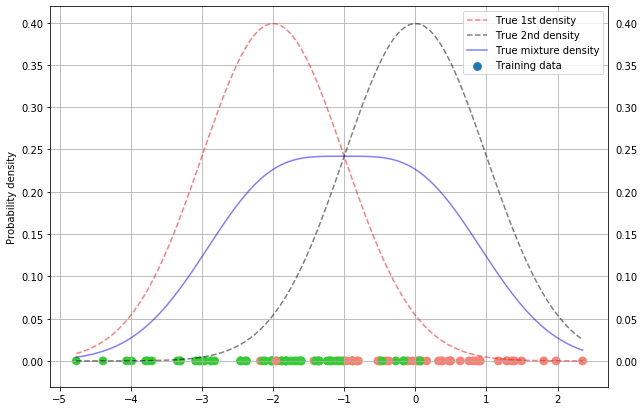
\includegraphics[scale=0.3]{mu0_mum2.png}
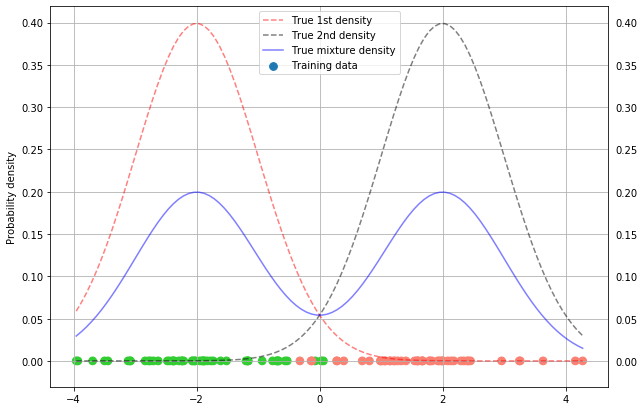
\includegraphics[scale=0.3]{mu2_mum2.png}
\caption{Samples and density when   $\mu_0 = -2$ et $\mu_1 = 0$ (left) and $\mu_0 = -2$ and $\mu_1 = 2$ (right).}
\end{center}
\end{figure}

\begin{enumerate}
\item Provide an expression of a classifier $h_*$ minimizing $h \mapsto \bP(h(X)\neq Y)$.

\vspace{.2cm}

{\em The classifier $h_*$ such that $h_{*}(X) = 1$ if and only if $\bP(Y=1|X)> \bP(Y=0|X)$ minimizes the missclassification error:
$$
h_{*} \in \mathrm{Argmin}_{h:\rset\to \{0,1\}}\left\{\bP(h(X)\neq Y)\right\}\eqsp.
$$
}

\item Using Bayes rule, show that  $h_*$ depends only on $g_1/g_0$.

\vspace{.2cm}

{\em  By Bayes formula, $\bP(Y=1|X) = \bP(Y=1)g_1(X)/g(X)$, which yields
$$
\frac{\bP(Y=1|X)}{\bP(Y=0|X)} = \frac{g_1(X)}{g_0(X)}\eqsp.
$$
Then, $h_*(X) = 1$ if and only if $g_1(X)/g_0(X)>1$.
}

\item Show that the Bayes classifier uses the mean between  $\mu_0$ and  $\mu_1$ to classify samples.

\vspace{.2cm}

{\em $h_*(X) = 1$ if and only if  $\log g_1(X) - \log g_0(X)>0$, so that, assuming without loss of generality that $\mu_1>\mu_0$:
\begin{align*}
h_*(X) = 1 & \Leftrightarrow (X-\mu_0)^2 - (X-\mu_1)^2>0\,,\\
& \Leftrightarrow 2 (\mu_1-\mu_0)X + \mu_0^2 - \mu_1^2>0\,,\\
&\Leftrightarrow X> \frac{\mu_1^2 - \mu_0^2}{2(\mu_1-\mu_0)}\,,\\
& \Leftrightarrow X> \frac{\mu_1 + \mu_0}{2}\eqsp.
\end{align*}
This criterion can lead to very poor performance if means are close (see Figure~1).}
\end{enumerate}



\section{Bayes classifier}
\subsection{Uniform distributions}
Assume that $(X,Y)\in\mathbb{R}\times\{0,1\}$ is defined on $(\Omega,\mathcal{F},\mathbb{P})$ with $\mathbb{P}(Y=1) = \pi \in(0,1)$.  Assume that conditionally on $\{Y=0\}$ (resp. $\{Y=1\}$) $X$ has a uniform distribution on $[0,\theta]$ with $\theta\in(0,1)$ (resp. on $[0,1]$). Compute $\eta(X) = \mathbb{P}(Y=1 |X)$.

\vspace{.2cm}

{\em
Let $g$ be the probability density function of $X$. For any measurable set $A$,
\begin{align*}
\mathbb{P}(X\in A) &= \mathbb{P}(Y=0)\mathbb{P}(X\in A|Y=0) + \mathbb{P}(Y=1)\mathbb{P}(X\in A|Y=1)\,,\\
&= (1-\pi) \theta^{-1}\int \1_A(x)\1_{[0,\theta]}(x) \rmd x + \pi \int \1_A(x)\1_{[0,1]}(x) \rmd x\,,\\
&= \int \1_A(x)\left\{ (1-\pi) \theta^{-1}\1_{[0,\theta]}(x) + \pi\1_{[0,1]}(x)\right\} \rmd x\,.
\end{align*}
Therefore, $g:x\mapsto  (1-\pi) \theta^{-1}\1_{[0,\theta]}(x) + \pi\1_{[0,1]}(x)$. Then, using Bayes rules and writing $g_1$ the probability density of the distribution of $X$ given $\{Y=1\}$,
$$
\eta(X) = \mathbb{P}(Y=1 |X) = \frac{ \mathbb{P}(Y=1)g_1(X)}{g(X)} = \frac{\pi \1_{[0,1]}(X)}{(1-\pi) \theta^{-1}\1_{[0,\theta]}(X) + \pi\1_{[0,1]}(X)}\eqsp.
$$

}

%\subsection{Exercice 2}
%Assume that $(X,Y)\in\mathbb{R}\times\{0,1\}$ is defined on $(\Omega,\mathcal{F},\mathbb{P})$. The distribution of $X$ is written $\mu$ and $\eta(X) = \mathbb{P}(Y=1|X) = X(X+\theta)^{-1}$ where $\theta>0$. Compute the Bayes classifier $h^*$ in this setting and prove that
%$$
%\mathsf{R}(h^*) = \bP(h^*(X)\neq Y) = \int \{\eta(x) \wedge (1-\eta(x))\}\mu(\rmd x)\,.
%$$
%Compute $R(h^*)$ when $\mu$ is the uniform distribution on $[0,\alpha \theta]$, $\alpha>1$. 

\subsection{Weighted risk}
Assume that $(X,Y)\in\mathbb{R}\times\{0,1\}$ is defined on $(\Omega,\mathcal{F},\mathbb{P})$. Using $\omega_0, \omega_1 >0$, with $\omega_0+\omega_1 = 1$, we  consider the weighted risk:
$$
\mathsf{R}(h) = \bE[2\omega_Y \mathds{1}_{Y\neq h(X)}]\,.
$$
Compute a classifier $h_*$ minimizing $h\mapsto \mathsf{R}(h)$ and $\mathsf{R}(h_*)$.

\vspace{.2cm}

{\em
For all classifiers $h$, writing $\eta(X) = \bP(Y=1|X)$,
\begin{align*}
\mathsf{R}(h) = \bE[2\omega_Y \mathds{1}_{Y\neq h(X)}] &= \bE[2\omega_Y \mathds{1}_{Y=1}\mathds{1}_{h(X)=0} + 2\omega_Y \mathds{1}_{Y=0}\mathds{1}_{h(X)=1}]\eqsp,\\ 
&= \bE[2\omega_1 \mathds{1}_{Y=1}\mathds{1}_{h(X)=0} + 2\omega_0 \mathds{1}_{Y=0}\mathds{1}_{h(X)=1}]\eqsp,\\ 
&= \bE[2\omega_1 \eta(X)\mathds{1}_{h(X)=0} + 2\omega_0 (1-\eta(X))\mathds{1}_{h(X)=1}]\eqsp,\\ 
\end{align*}
Therefore, choosing $h_\star:x\mapsto \mathds{1}_{\omega_1 \eta(X)\geqslant \omega_0 (1-\eta(X))}$ yields,
$$
\mathsf{R}(h) \geqslant \mathsf{R}(h_*)\eqsp. 
$$
Then, by definition, for all $x\in\mathbb{R}^d$,
$$
h_\star(x) = 1 \Leftrightarrow \omega_1 \eta(x) \geqslant \omega_0 (1-\eta(x))
$$
and 
$$
2\omega_1 \eta(x)\mathds{1}_{h_*(x)=0} + 2\omega_0 (1-\eta(x))\mathds{1}_{h_*(x)=1} = 2 \left(\omega_1 \eta(x)\right) \wedge \left(\omega_0 (1-\eta(x))\right)\eqsp.
$$
This yields
$$
\mathsf{R}(h_*) = 2\bE[ \left(\omega_1 \eta(X)\right) \wedge \left(\omega_0 (1-\eta(X))\right)]\eqsp.
$$
}


\section{Additional exercises}

\subsection{Bayes classifier: excess risk}
Let $(X,Y)\in\rset^d\times\{0,1\}$ be random variables defined on the same probability space $(\Omega,\calF,\bP)$.
For any classifier $h:\mathcal{X}\to \{0,1\}$, define its classification error by
$$
\mathsf{R}(h)=\bP(Y\neq h(X))\eqsp.
$$
The classifier $h_*$ defined by:
$$
h_{*}(x)={\rm sign}(\eta(x)-1/2)\eqsp,
$$
where
$$
\eta(X) = \bP(Y=1|X)\eqsp,
$$
minimizes $h\mapsto \mathsf{R}(h)$.
\begin{enumerate}
\item Prove that 
$$
\mathsf{R}(h_*) = \mathbb{E}\left[\eta(X) \wedge (1-\eta(X))\right]\leqslant \frac{1}{2}\eqsp.
$$

\vspace{.2cm}

{\em
For all classifiers $h$, as $h$ and $Y$ take values in $\{0,1\}$,
$$
\mathsf{R}(h) = \mathbb{E}\left[\1_{h(X)\neq Y}\right] = \mathbb{E}\left[h(X)(1-Y) + (1-h(X))Y\right]\eqsp.
$$
As $\mathbb{E}[Y|X] = \eta(X)$ this yields,
$$
\mathsf{R}(h) = \mathbb{E}\left[h(X)(1-\eta(X)) + (1-h(X))\eta(X)\right]
$$
and 
$$
\mathsf{R}(h_*) = \mathbb{E}\left[h_*(X)(1-\eta(X)) + (1-h_*(X))\eta(X)\right] =  \mathbb{E}\left[\eta(X) \wedge (1-\eta(X))\right]\eqsp.
$$
}
\item Prove that for all classifiers $h$, the excess risk is given by
$$
\mathsf{R}(h)  - \mathsf{R}(h_*) = \mathbb{E}\left[\left|1-2\eta(X)\right|\left|h(X) - h_*(X)\right|\right]\eqsp.
$$

\vspace{.2cm}

{\em
By the previous question, for all classifiers $h$,
\begin{align*}
\mathsf{R}(h)  - \mathsf{R}(h_*) &= \mathbb{E}\left[(h(X) - h_*(X))(1-\eta(X)) + (h_*(X)-h(X))\eta(X)\right]\eqsp,\\
 &= \mathbb{E}\left[(h(X) - h_*(X))(1-2\eta(X))\right]\eqsp.
\end{align*}
By definition of $h_*$, $h(X) - h_*(X)$ and $1-2\eta(X)$ have the same sign so that
$$
\mathsf{R}(h)  - \mathsf{R}(h_*) = \mathbb{E}\left[\left|1-2\eta(X)\right|\left|h(X) - h_*(X)\right|\right]\eqsp.
$$
}
\end{enumerate}



\subsection{Plug-in classifier}
Let $(X,Y)\in\rset^d\times\{-1,1\}$ be random variables defined on the same probability space $(\Omega,\calF,\bP)$.
For any classifier $h:\mathcal{X}\to \{-1,1\}$, define its classification error by
$$
\mathsf{R}(h)=\bP(Y\neq h(X))\eqsp.
$$
The classifier $h_*$ defined by:
$$
h_{*}(x)={\rm sign}(\eta(x)-1/2)\eqsp,
$$
where
$$
\eta(X) = \bP(Y=1|X)\eqsp,
$$
minimizes $h\mapsto \mathsf{R}(h)$. Given $n$ independent couples $\{(X_i,Y_i)\}_{1\leqslant i \leqslant n}$ with the same distribution as $(X,Y)$, an empirical surrogate for $h_{*}$ is obtained from a possibly nonparametric estimator $\widehat \eta_n$ of $\eta$:
$$
\widehat h_n: x\mapsto {\rm sign}(\widehat \eta_n(x)-1/2)\eqsp.
$$
\begin{enumerate}
\item Prove that for any classifier $h:\mathcal{X}\to \{-1,1\}$,
$$
\bP(Y\neq h(X)|X) = (2\eta(X)-1)\1_{h(X)=-1}+1-\eta(X)
$$
and
$$
\mathsf{R}(h)-\mathsf{R}(h_{*})=2\bE \left[\left|\eta(X)-\frac{1}{2}\right|\eqsp\1_{h(X)\neq h_*(X)}\right]\eqsp.
$$

\vspace{.2cm}

{\em
For all classifiers $h$,
\begin{align*}
\bP\left(Y \neq h(X) | X\right)& = \bP\left(Y=-1, h(X) = 1 |X\right) + \bP\left(Y=1, h(X) = -1 |X\right)\eqsp,\\
& = \1_{h(X) = 1} \bP\left(Y=-1 |X\right) + \1_{h(X) = -1} \bP\left(Y=1 |X\right)\eqsp,\\
& = \1_{h(X) = -1} (2\eta(X) - 1) + 1 - \eta(X)\eqsp.
\end{align*}
Then,
$$
\mathsf{R}(h)-\mathsf{R}(h_{*})=\bE \left[\left(\1_{h(X) = -1}-\1_{h_*(X) = -1}\right) (2\eta(X) - 1) \right] =  2\bE \left[\left|\eta(X)-\frac{1}{2}\right|\eqsp\1_{h(X)\neq h_*(X)}\right]\eqsp.
$$
}
\item Prove that 
$$
|\eta(x)-1/2|\1_{\widehat h_n(x)\neq h_{*}(x)}\leqslant |\eta(x)-\widehat \eta_n(x)|\1_{\widehat h_n(x)\neq h_{*}(x)}\eqsp,
$$
where
$$
\widehat h_n:x \mapsto{\rm sign}(\widehat \eta_n(x)-1/2)\eqsp.
$$
Deduce that 
$$
\mathsf{R}(\widehat h_n)-\mathsf{R}(h_*)\leqslant  2 \bE[|\eta(X) - \widehat \eta_n(X)|^2]^{1/2}\eqsp.
$$

\vspace{.2cm}

{\em
Note that, for all $x\in\mathbb{R}^d$, $\widehat h_n(x) \neq h_*(x)$ if and only if i) $\eta(x) > 1/2$ and $\widehat\eta_n(x) \leqslant 1/2$ or ii) $ \eta(x) \leqslant 1/2$ and $\widehat \eta_n(x) > 1/2$. If $\eta(x) > 1/2$ and $\widehat\eta_n(x) \leqslant 1/2$, then $|\eta(x) - \widehat\eta_n(x)| = \eta(x) - \widehat\eta_n(x) \geqslant \eta(x) -1/2$. On the other hand, if $\eta(x) \leqslant 1/2$ and $\widehat \eta_n(x) > 1/2\}$, $|\eta(x) - \widehat\eta_n(x)| = \widehat\eta_n(x) - \eta(x) \geqslant 1/2 - \eta(x)$. 
Therefore, for all $x\in\mathbb{R}^d$,
$$
|\eta(x) - 1/2| \1_{\widehat h_n(x) \neq h_*(x)}\leq |\eta(x) - \widehat \eta_n(x)| \1_{\widehat h_n(x) \neq h_*(x)}\eqsp.
$$
By the first question and Cauchy-Schwarz inequality, 
\begin{align*}
\mathsf{R}(\widehat h_n) - \mathsf{R}(h_*) & = 2  \bE \left[ \left| \eta(X) - 1/2 \right| \1_{h_*(X) = \widehat h_n(X)}  \right]\eqsp,\\
& \leqslant 2 \bE \left[ \left|\eta(X) - \widehat \eta_n(X) \right| \1_{\widehat h_n(X) \neq h_*(X)}  \right]\eqsp,\\
& \leqslant 2 \bE[|\eta(X) - \widehat \eta_n(X)|^2]^{1/2}\eqsp.
\end{align*}
}
\end{enumerate}



\end{document}